For relevant nuclear forensics predictions, both classification and regression
algorithms must be used.  For example, one may want to predict the reactor type
based on some measurements (referred to as features) of spent fuel of an
unknown source, and this would require a classification algorithm. Or perhaps
the input fuel composition is relevant to an investigation on weapons intent,
so a regression algorithm would be used to train a model based on some set of
features.  Since this work trains models to predict burnup of \gls{SNF}, the 
algorithms are presented in a regression context.

\subsubsection{Linear Models}
\label{sec:linear}

One of the simplest and most utilized methods of prediction is a linear model
from a least-squares fit. Thus, it is the most natural place to begin a
demonstration of machine learning algorithms. Since linear models must have all
parameters linearly related, there are many restrictions regarding the shape of
the model. However, this makes the resulting models stable to peturbations. 

An example of a linear model is below, where the vector of input features of
size $p$, $\boldsymbol{X}$, provides a model, $F(\boldsymbol{X})$ ($Y$ is the
known model), by determining the unknown coefficients, or weights,
$\beta_{j}$'s. The algorithm calculates these by minimizing the value of a loss
function over all the training data.  This is usually the least squares error
from minimizing the sum of squared errors, $\sum_{i=1}^{n} (y_i - f(x_i))^2$.
But it could instead be the least absolute deviations from minimizing the sum
of absolute error differences, $\sum_{i=1}^{n} |y_i - f(x_i)|$. These are
referred to as the $L_2$ and $L_1$ norms, respectively.  

\begin{equation}
  F(\boldsymbol{X}) = \beta_{0} +  \sum_{j=1}^{p} x_{j} \beta_{j}
\end{equation}

\begin{figure}[!htb]
  \centering
  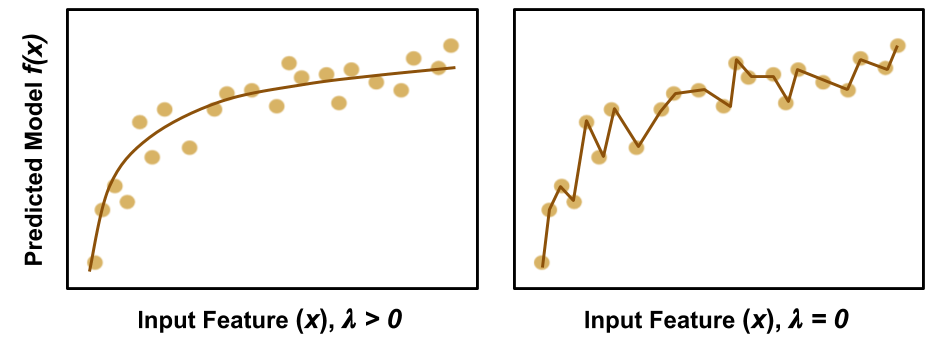
\includegraphics[width=\linewidth]{./chapters/litrev/regularization.png}
  \caption{Illustrtation of the effect of regularization on model prediction}
  \label{fig:reg}
\end{figure}

The form of linear regression used here is called ridge regression. This
algorithm performs optimization using the $L_2$ norm, and also uses the form of
the $L_2$ norm for \textit{regularization}. Regularization, sometimes called
\textit{shrinkage}, is a term introduced into the predicted model to prevent
overfitting. (It is used in many machine learning algorithms.) This works by
further reducing the weights, $\beta_j$, on the input features, $x_j$. This
shrinkage term also includes a complexity parameter, $\lambda$
\cite{elements_stats}.  Thus, the predicted linear model from ridge regression
is updated to the following equation.  A visualization of what this
regularization can accomplish is in Figure \ref{fig:reg}.

\begin{equation}
  F(\boldsymbol{X}) = \beta_{0} +  \sum_{j=1}^{p} x_{j} \beta_{j} + \lambda \sum_{j=1}^{p} \beta_{j}^2
\end{equation}

\subsubsection{Nearest Neighbor Methods}
\label{sec:neighbor}

Nearest neighbor regression is considered to be `model-free' in that it does
not actually generalize; it tracks the observations in the training set.
During prediction, the algorithm will calculate a value based on the instance
that is closest to the current test sample. Thus, there is not any learning,
but instead a direct comparison between an unknown sample and the space that
the training set populates. The predictions from nearest neighbors can be quite
accurate, but are highly unstable to peturbations \cite{elements_stats}.  

An extension of nearest neighbor is \textit{k}-nearest neighbor regression.
The closest \textit{k} neighbors are averaged to provide an estimate of the
unknown sample. The equation below shows how this algorithm does this to
determine a predict a value, $Y$, from the input features, $\boldsymbol{X}$, in
the neighborhood, $N_k (\boldsymbol{X})$ \cite{elements_stats}.  

\begin{equation}
  Y(\boldsymbol{X}) = \frac{1}{k} \sum_{x_i \in N_k(\boldsymbol{X})} y_i
\end{equation}

A measure of distance dictates what the neighborhood is. The metrics for
distance differ, but in this study, the Euclidian distance was used. Another
parameter is the population of the neighborhood, \textit{k}. In this initial
work, $k = 1$ is used. This can perform very well, but can also easily overfit
the data and thus not generalize well. 

\subsubsection{Support Vector Machines}
\label{sec:svm}

\gls{SVR} is an extension of the popular classification algorithm, \gls{SVM}.
This algorithm was chosen because of its ability to handle highly dimensional
data well, which in this study is a maximum of approximately 300 features. 

As seen in Figure ?, the \gls{SVM} algorithm separates two classes by
determining an optimal hyperplane, given by $wx+b = 0$, between them. The
algorithm evaluates the quality of the line that separates the two classes by
maximizing the margin width, $w$, given the constrains of the surrouding lines.
Some problems are not linearly separable, and thus a penalty term, $\xi$, is
introduced to allow for misclassifications. As shown in Figure ?, the algorithm
then simultaneously minimizes the misclassifications while maximizing the
margin. 

This can be extended easily to multidimensional analysis via what is called the
\textit{kernel trick}.  First, using a nonlinear kernel function maps the data
into higher dimensional feature space. Then the algorithm can find a linear
separation in this space, as shown in Figure ?. Further, this can be upgraded
from classification to SVR by doing similar math but instead minimizing the
margin, as shown in Figure ?. 

The kernel chosen for this study is the Gaussian radial basis function, shown
below. This has two tuneable parameters, gamma and C. Gamma influences the
width of influence of individual training instances, and strongly affects the
fitting of the model. Low values correspond to underfitting because the
instances have too large of a radius (low influence) and high values correspond
to overfitting because the instances have a small radius (high influence). 

The C parameter also affects the fitting of the model by allowing more or less
support vectors, corresponding to more or less misclassification. A lower C
smooths the surface of the model by allowing more misclassifications, whereas a
higher C classifies more training examples by allowing fewer
misclassifications. Too low and too high of a C can cause under- and
overfitting, respoectively. 

Since there is a tradeoff of fitting strength provided by both parameters, it
is common to run the algorithm on a logarithmic grid from 10'-3 to 10'3 for
each parameter. If plotted on a heatmap of accuracies given gamma and C, there
will be a diagonal of ideal combinations that emerges. The lowest of these is
usually chosen. 

